\subsubsection{Entrop\'ia de Shannon}
\label{sec:Entriopia}
    La entrop\'ia de Shannon es un concepto fundamental en la teor\'ia de la informaci\'on, 
        que se utiliza para medir la incertidumbre en una variable aleatoria. La entriop\'ia en si 
        es el grado de informaci\'n/desinformaci\'on que tenemos en un sistema. Es decir que cuanta m\'as
        informaci\'on tengamos de un sistema, menor ser\'a la entrop\'ia y viceversa. La entrop\'ia de Shannon, 
        nombrada as\'i por Claude Shannon\cite{Shannon}, se define mate la suma negativa de las probabilidades de cada
        posible valor de la variable aleatoria multiplicada por el logaritmo de la probabilidad de ese valor. Esta
        definici\'on es la siguiente:
        \begin{equation}
            H(X) = -\sum_{i=1}^{n} p(x_i) \log_b p(x_i)
        \end{equation}
    \vskip 0.5cm
    Donde $X$ es una variable aleatoria discreta, $p(x_i)$ es la probabilidad de que la variable aleatoria 
        $X$ tome el valor $x_i$ y $b$ es la base del logaritmo. En el caso de que la base del logaritmo sea 2, 
        la unidad de medida de la entrop\'ia ser\'an los bits. En el caso de que la base del logaritmo sea $e$,
        la unidad de medida de la entrop\'ia ser\'an los nat. Y en el caso de que la base del logaritmo sea 10, 
        la unidad de medida de la entrop\'ia ser\'an los dits.
    \vskip 0.5cm
    En nuestro caso en particular usamos bits como unidad de medida de la entrop\'ia, ya que lo usamos para saber que tipo de comportamiento
        tiene el aut\'omata celular. Es decir, si la entrop\'ia es alta, entonces el aut\'omata celular tiene un comportamiento ca\'otico, y si 
        la entrop\'ia es baja, entonces el aut\'omata celular tiene un comportamiento ordenado.
    \vskip 0.5cm
    Como vimos en ejemplo anterior, el aut\'omata celular \textit{Anneal} podemos observar r\'apidamente su entriop\'ia
        en la figura \ref{fig:annealEntropia}: 
        \begin{figure}[h]
            \centering
            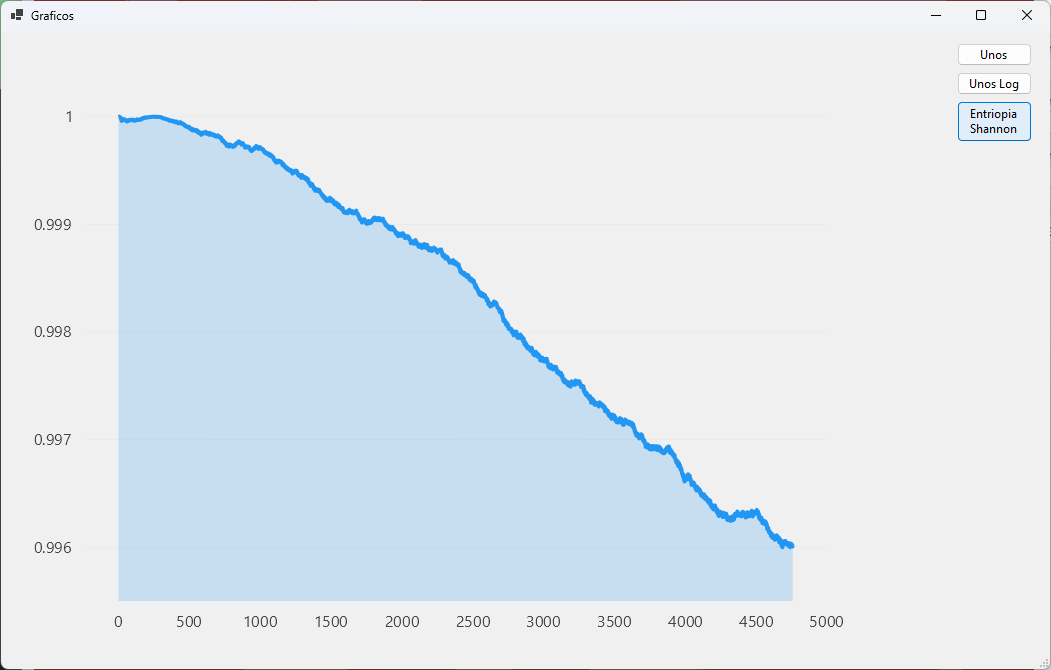
\includegraphics[width=0.5\textwidth]{./images/marco_teorico/automatas_celulares/Anneal5kShann.png}
            \caption{Entrio\'ia del aut\'omata celular \textit{Anneal} en 5000 generaciones}
            \label{fig:annealEntropia}  
        \end{figure}